%%%%%%%%%%%%%%%%%%%%%%%%%%%%%%%%%%%%%%%%%%%%%%%%
%
% This is a template file
%
% Copy it to a new file with a new name and use it as the basis
% for your article
%
%%%%%%%%%%%%%%%%%%%%%%%%%%

\documentclass[EPJ,twocolumn]{webofc}
\usepackage[varg]{txfonts}   
\usepackage{float}
\usepackage{fancyhdr}

\setlength\headheight{26pt}

\lhead{
\includegraphics[width=1.5cm]{LIP.png}}

%PAGE NUMBER (should appear after first page)
\rhead{\thepage}

% Add here some packages that may be required 
\usepackage{hyperref}

% Add here some personal commands if needed
\newcommand{\bbar}{\ensuremath{\text{b}\overline{\text}}}

% This specifies the reference of each report
% this will be further specified later on 
\wocname {\texttt{LIP-STUDENTS-23-00}}
\woctitle{\texttt{LIP-STUDENTS-23-00}}

\title{Predicting COMPASS/AMBER Acceptance Using Neural Networks}

\author{Pedro Curvo\inst{1} \fnsep\thanks{\email{pedro.curvo@tecnico.ulisboa.pt}} 

\institute{
Instituto Superior T\'ecnico, Lisboa, Portugal
\vskip 2mm
{\normalfont\normalsize\textsf Project supervisor: Marcin Stolarski}
\mbox{}\hfill\today\hspace*{16mm}
}

\abstract{A review on a reported search of the Standard Model (SM) Higgs boson decaying to a $\text{b}\overline{\text{b}}$ pair when produced along an electroweak vector boson is made. The search was performed using data samples recorded from Run 2 of the LHC by the CMS experiment in 2016. The CMS experiment and the importance of the search for this decay are briefly discussed. Branching ratios of several Higgs boson decays are presented. The methods used to analyse the data samples are discussed as well, namely how can objects be reconstructed, the experimental procedure for the 0-lepton channel, and strategies adopted to suppress background events. The results of the observed signal events are consistent with the SM predictions.

% Keywords: avoid repeating title
\vskip 2mm
{\textsc{Keywords:} LHC, Higgs, branching fraction}
}


% The actual document starts here
\begin{document}

\maketitle

\section{Introduction}
\label{sec:intro}
\subsection{The CMS detector}
The CMS detector (Compact Muon Solenoid) is one of the detectors from the LHC, at CERN. It has a cylindrical shape and consists on a central region where the collisions occur, followed by a silicon tracker which tracks the passage of charge particles (which curve in opposite directions for particles with opposite charge), then an electromagnetic calorimeter, where photons and electrons typically lay their energy in the form of energy clusters (showers) and an hadronic calorimeter, where hadrons deposit their energy. Continuing outwards, there is the superconducting solenoid which produces the 3.8 T magnetic field and the muon chambers, with up to four stations of gas-ionization muon detectors installed outside the solenoid and sandwiched between the layers of the steel return yoke (a full description can be found in \cite{cmsdetector}).

\begin{figure}[H]
\centering
\sidecaption
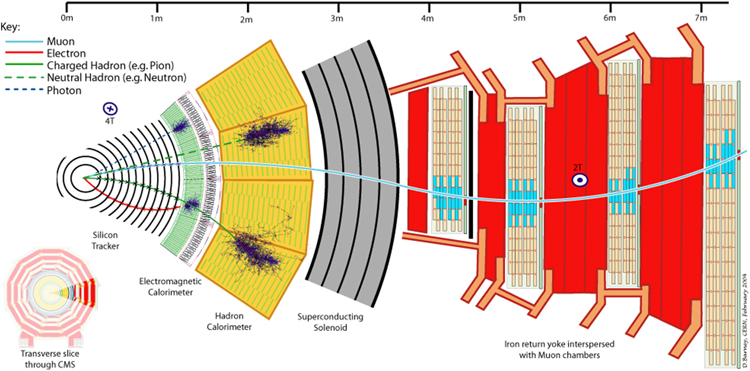
\includegraphics[width=0.45\textwidth,clip]{img/scheme_transverse_cms.jpg}
\caption{Schematic transverse view of the CMS detector}
\label{figure1}       
\end{figure}

\subsection{Relevant variables}

Here we present a list of the main variables which can be measured with the detector and are used in this analysis.

\begin{itemize}
    \item   $\theta$ : polar angle of the trajectory of a particle with respect to the counterclockwise proton beam;
    \item     $\eta$ = $-\ln(\tan \theta/2)$ : pseudorapidity;
    \item     $\phi$ : angle of the trajectory of the object in the plane transverse to the direction of the proton beams;
    \item  $\Delta R =  \sqrt{(\Delta \eta)^2 - (\Delta \phi)^2}$ : separation between reconstructed objects in the detector;
    \item $p_T$ : transverse momentum;
    \item $p_T^{miss}$ : missing transverse momentum - magnitude of the negative vector sum of the transverse momenta of all reconstructed objects;
    \item $H_T^{miss}$ : hadronic missing transverse momentum - magnitude of the negative vector sum of the transverse momenta of all reconstructed jets (with $p_T$ > 20 GeV and $|\eta|$ < 5.2).
    \item $M$ : invariant mass;
    \item $N$ : number of objects (example: $N_{aj}$ is the number of additional jets)
\end{itemize}


\subsection{The $\text{H} \rightarrow \text{b}\overline{\text{b}}$ decay}
%este pedaço foi o ninhos

The article this paper reviews \cite{artigo} reports the search of the Higgs boson decay into \bbar\, when produced through the $\text{pp} \rightarrow \text{VH}$ process, where V designates a vector W or Z boson. This search was done using data samples from Run 2 of the LHC, recorded during 2016, with an integrated luminosity of 35.9 fb$^{-1}$ and center of mass energy of $\sqrt{s}=13$ TeV. The processes considered in this search are  $\text{Z}(\nu \nu)\text{H}$, $\text{W}(\mu \nu)\text{H}$, $\text{W}(e \nu)\text{H}$, $\text{Z}(\mu \mu)\text{H}$ and $\text{Z}(ee)\text{H}$. The final states of the vector boson decay are caracterized by their number of leptons, corresponding a channel to each number. So there are three channels under consideration, the 0-lepton, the 1-lepton and 2-lepton channels. In this paper, lepton (represented by $\ell$) designates solely a muon or an electron, once the leptonic tau decays in WH and ZH processes are implicitly included in the five processes mentioned.
In which regards the Higgs boson decay, there are several background sources that enhance the complexity of the data analysis. These sources originate from the production of vector bosons in association with W+jets (from gluons), Z+jets (from light or heavy flavoured quarks), from singly and pair produced top quarks (single t or $\text{t}\overline{\text{t}}$), from diboson production (VV) and from QCD multijet events. Unfortunately, most of these processes have cross sections several orders of magnitude larger than the one of the Higgs boson production. Hence, the stratigies adopted to overcome these problems are discussed in Section~\ref{sec:bckgr}.



\section{Branching ratios}
%este pedaço foi o ninhos
A correct treatment and interpretation of the data acquired demands high precision on the predicted decay widths and their uncertainties. 
As until the discovery of the particle its mass was unknown, several efforts were made to calculate the partial widths, and thus, the branching ratios, of all the relevant decays of the Higgs boson, either to 2-particle (pairs of bosons or of leptons) or to 4-particle final states (which include decays into leptons, semi-leptons or hadrons), at least up to NLO, considering both electroweak and QCD corrections, in multiple mass ranges (\cite{handbook1,higgsproperties}).
In the figures \ref{higgsbr1} and \ref{higgsbr2} we can follow the variation of the branching ratios of the bosonic and fermionic decays with the particle's mass, in the low mass and full mass ranges, respectively.

\begin{figure}[H]
\centering
\sidecaption
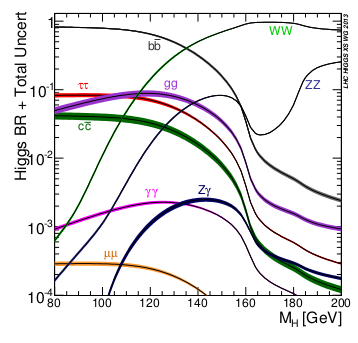
\includegraphics[width=0.3\textwidth,clip]{img/lowmassrange.png}
\caption{Higgs branching ratios, including uncertainties, in the low mass range.}
\label{higgsbr1}       
\end{figure}

\begin{figure}[H]
\centering
\sidecaption
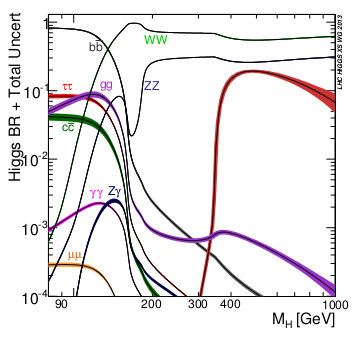
\includegraphics[width=0.3\textwidth,clip]{img/fullmassrange.png}
\caption{Higgs branching ratios, including uncertainties, in the full mass range.}
\label{higgsbr2}       
\end{figure}

These plots were useful for the search of the Higgs boson (\cite{bworld}), as they show the channels one should look at, depending on the mass range.
The b$\overline{\text{b}}$ channel is of particular interest as it tests directly the Higgs boson coupling to fermions, ensuring it as the mass generation source in the fermion sector of the SM.
At first sight, one would think that in the low mass range the search for the Higgs boson should be done using data from the b$\overline{\text{b}}$ channel, and from the ZZ and WW channels in the high mass range. However, the background events can difficult the detection of the boson in these channels, and other channels must be taken into account, namely those which don't include hadronic final states. Some considered decays were the $\gamma\gamma$ and the 4-particle final states $\ell \ell \ell \ell $ or $\ell \nu \ell \nu$.


\section{Object Reconstruction}

The caracterization of the VH events requires the reconstruction of several objects, namely muons, electrons, neutrinos (indentified by the missing transverse momentum, $p_{T}^{miss}$) and jets, originating from the primary interaction vertex. The primary pp interaction vertex is taken to be the one with the largest value of summed physics-object $p_{T}^2$.
The objects are identified by using a particle flow (PF) algorithm.

\subsection{Leptons}

\subsubsection*{Electrons}
Electrons are reconstructed by matching a set of clusters of energy deposited in the electromagnetic calorimeter (ECAL), denoted supercluster (SC), with tracks in the silicon tracker and applying a multivariate technique, which is a computational tool that combines multiple variables, analysing correlations between them and producing one output. This technique in particular combines the information from observables like geometric matching and momentum consistency between the electron trajectory and the associated calorimeter clusters, as well as the shower shapes in the calorimeter. Besides that, there is the need to impose additional cuts to avoid considering electrons that originate from photon conversions and not from the interaction vertex. In particular, electrons are required to have $|{\eta}| < 2.5$, and candidates for which $1.444 < |\eta_{SC}| < 1.566$ (transition region between the ECAL barrel and the endcap) will be excluded because the electron reconstruction is not optimal in this area.

\subsubsection*{Muons}

Muons will be reconstructed by matching tracks in the silicon detector with ionizations in the muon chamber, using two algorithms.

The first one matches tracks in the silicon tracker with hits in the muon detectors, and the other performs a track fit between the hits in these two detectors. A candidate is identified as a muon if it is successfully reconstructed by both algorithms. To reduce misidentification, the tracks must also obey other criteria like compatibility between the number of hits in the tracker and in the muon systems, the fit of the global muon track and its consistency with the primary vertex. Muon candidates are also required to be in the $|\eta|$ < 2.4 region.

For both electrons and muons there is yet another criterium called the isolation. Charged leptons which come from a W or Z boson decay are expected to be isolated from other aspects of the event. For each lepton candidate a $\eta-\phi$ cone is built around the track direction and the sum of the transverse momentum of all reconstructed particles (from the primary vertex) within the cone, except from the contribution of the lepton itself, is calculated. This sum is the isolation. In the presence of pileup, this quantity is contamined with particles from other interactions, therefore a quantity proportional to the pileup is used to correct the isolation.

In the 1-lepton channel, if the corrected isolation sum exceeds 6\% of the lepton candidate $p_T$, the lepton is rejected. In the 2-lepton channel, this threshold is 20\% for muons and 15\% for electrons. The total efficiency for reconstructing muons is in the
range of 85–100\%, and for electrons it's in the range of 40–90\%.

\subsection{Jets}

Jets are reconstructed from particle-flow (PF) objects using the anti-$k_T$ clustering algorithm. Each one must lie within $|\eta|<2.4$, to have at least two tracks associated with it, and to have electromagnetic and hadronic energy fractions of at least 1\%. Energy corrections are applied as a function of  $|\eta|$ and $p_T$ of the jet. The 3-momentum $\vec{p}_{T}^{miss}$ is determined offline by the negative of the vectorial sum of transverse momenta of all PF objects identified in the event.


We need to point out that pileup interactions affect jet momentum reconstruction and b tagging efficiencies. To overcome this problem, all charged hadrons that do not originate from the primary interaction vertex are removed from consideration in the event. In addition, the average neutral energy density from pileup interactions is evaluated from PF objects and subtracted from the reconstructed jets in the event and from the summed energy in the isolation criteria used for leptons.


\subsubsection*{b-jets}

The jets that originate from the hadronization of b quarks, b-jets, are identified with a combined multivariate (CMVA) b tagging algorithm, which helps differentiate between b-jets and jets originating from light quarks, gluons or charm quarks. By combining certain informations within the jet, as track impact parameters, secondary vertices, and information related to low-$p_T$ leptons, the algorithm gives an output value between -1.0 and +1.0, which is called the CMVA discriminant. If it lies above a certain chosen threshold, the jet is labeled as "b-tagged". The tagging efficiency depends on the value of the threshold, which is parametrized according to the $p_T$ and $\eta$ values of the jet.

The reconstruction of the $\text{H} \rightarrow \text{b}\overline{\text{b}}$ decay is done by selecting a pair of jets that have the highest value of CMVA discriminant among all other jets in the event. Both jets are required to be central, i.e., with $|\eta|$<2.4, to satisfy standard requirements to remove jets from pileup, and to have a  $p_{T}$ above a certain threshold, that can be different for each jet.


\section{Experimental procedure}

Simulated samples of signal and background processes are produced using Monte Carlo event generators and are used to optimise the search.
The simulated samples include the several pp interactions per bunch (approx. 23), referred to as pileup interactions (or pileup), that overlap with the event of interest in the same bunch crossing.

\subsection*{Trigger}

Several triggers are applied to select events in which the final-state objects are consistent with the ones from the channels presented above. In this review we will concentrate on the experimental procedure for the 0-lepton channel.

For this channel, the PF algorithm is used to reconstruct the individual particles emerging from the proton proton collisions, using the online information from all CMS subsystems. The main trigger requires $p_T^{miss}$ and $H_T^{miss}$ above 110 GeV.

For Z($\nu\nu$)H events with
$p_T^{miss}$ > 170 GeV, evaluated offline, the trigger efficiency is approximately 92\%, and near 100\%
above 200 GeV.

\subsection*{Event selection}

The events which pass the trigger are submitted to further event selection. Signal events are characterised by the presence of a vector boson recoiling against two b jets with an invariant mass near 125 GeV. The event selection therefore relies on the reconstruction of the decay of the Higgs boson into two b-tagged jets and on the reconstruction of the leptonic decay modes of the vector boson. In the case of the 0-lepton channel, the requirements for signal selection are presented in the table above.

\begin{table}[H]
    \centering
    \caption{Criteria for event selection in the 0-lepton channel.}
    \label{evt_selection}
    \begin{tabular}{c|c}
        \hline
        Variable & (GeV) \\ \hline
        $p_T$(V) & >170 \\
        $p_T(\text{j}_1)$ & >60 \\
        $p_T(\text{j}_2)$ & >35 \\
        $p_T(\text{jj})$ & >120 \\
        $M(\text{jj})$ & [60,160] \\
        CMVA$_{max}$ & >CMVA$_T$ \\
        CMVA$_{min}$ & >CMVA$_L$ \\
        $N_{aj}$ & <2 \\
        $N_{al}$ & =0 \\
        $p_T^{miss}$ & >170 \\
        $\Delta \phi (\vec{p_T^{miss}},\text{j})$ & >0.5 \\
        $\Delta \phi (\vec{p_T^{miss}},\vec{p_T^{miss}}(\text{trk}))$ & <0.5 \\
        Event BDT & >-0.8 \\\hline
    \end{tabular}
\end{table}

This channel targets mainly Z($\nu\nu$)H events in which the $p_T^{miss}$ is interpreted as the transverse
momentum of the Z boson in the $\text{Z} \rightarrow \nu\overline{\nu}$ decay. The selection imposes a high value of $p_T^{miss}$ and a significant angular distance between this momentum and the jet, in order to avoid QCD multijet backgrounds. A different missing transverse momentum reconstruction is used (trk), in order to further reduce this background source. This momentum should be aligned with $p_T^{miss}$ within 0.5 radians. To reduce background events from t$\overline{\text{t}}$ and WZ production channels, events with any additional isolated leptons with pT > 20 GeV are rejected. The number of these additional leptons is denoted by $N_{al}$.

After this selection, to further improve the resolution of the dijet invariant mass of the two b jets from the Higgs boson decay (which is approximately 15\% at this point), there is a multivariate regression technique which is applied. This technique is similar to the ones applied for Run 1 in several $\text{H} \rightarrow \text{b} \overline{\text{b}}$ analyses by ATLAS and CMS (\cite{higgsatlas},\cite{higgscms}). This regression makes an estimate that provides a correction to the energy of each individual b jet, which is added to the already mentioned jet energy correction. This correction is computed using a Boosted Decision Tree (BDT, \cite{bdt}), which is trained on b jets from $\text{t}\overline{\text{t}}$ simulated events (which contains information on the jet structure, which is different for jet that originate from b quarks and from light-flavour quarks or gluons). Jets that come from b quarks typically contain more leptons and more missing energy (due to semileptonic b hadron decays) and other differentiating characteristics, like the distance between the decay and the primary vertex (which is longer for b quarks).

Furthermore, an event BDT discriminant is trained using simulated samples for signal and all background processes. The variables fed to the BDT are chosen by iterative optimization from a large number of potentially discriminating variables. Some of the most discriminating variables are $M(\text{jj})$, the number of additional jets, $N_{aj}$, the value of CMVA for the jet with the second-highest CMVA value, CMVA$_{min}$, and the distance between the two jets, $\Delta R(\text{jj})$.

Finally, the systematic uncertainties are carefully studied, and their combined effect results in a 25\% reduction of the expected significance for the SM Higgs boson rate.

\section{Background control strategies}
\label{sec:bckgr}

In the search for the  $\text{H} \rightarrow \text{b}\overline{\text{b}}$ decay,  regarding data analysis, the background processes mentioned in the first section must be taken into account. Son, for each channel, a region enriched with VH events is defined. The simulated samples in this region are used to train the BDT event discriminant mentioned in the last section to help distinguish between signal and background events. Several control regions, enriched in events from individual background processes, have also been selected for each channel. These regions were used to see if the data agrees with the simulated samples, and to provide a distribution to be later used for the signal extraction fit. 
As what has already been stated, the event selection  relies on the reconstruction of the decay of the Higgs boson into two b-tagged jets and on the reconstruction of the leptonic decay modes of the vector boson. Although the background from V+jets and diboson production is reduced significantly after b-tagging, there is the need to suppress additional background events on the signal region. To provide additional suppression of background events, specific requirements are imposed for each channel after the $\text{H}  \rightarrow \text{b}\overline{\text{b}}$ decay reconstruction. 

The 0-lepton channel has already been discussed.

%, the criteria of the event selection to supress background was already discussed in the last section.

The 1-lepton channel targets mainly W$(\ell \nu)$H events, identifying the $\text{W} \rightarrow \ell \nu$ decay by the presence of one isolated lepton and $p_{T}^{miss}$ . The muons/electrons are required to have $p_{T}$> 20/30 GeV. It is also required that the azimuthal angle formed between $\vec{p}_{T}^{miss}$ and the lepton to be less than 2.0 radians. The lepton isolation for either flavor of lepton is required to be smaller than 6\% of the lepton $p_{T}$. Events with additional isolated leptons are also rejected in this case. To diminish effectively the background of $\text{t}\overline{\text{t}}$ events, $N_{aj}$ with $\eta$<2.9 and $p_{T}$>25 Gev must be no greater than one.

The 2-lepton channel targets $\text{Z} \rightarrow \ell \ell$ decays, which are reconstructed by combining isolated and oppositely directioned pairs of electrons/muons, requiring the invariant mass to satisfy $75< M(\text{jj})<105$ GeV. The $p_{T}$ for each lepton is required to be greater than 20 GeV. The requirements on this channel are looser, once QCD multijet background is practically eliminated after requiring compatibility with the Z boson mass.

The measurement of the hadronic activity associated with the main primary vertex provides an additional discriminating variable to reject background. The hadronic activity is measured by reconstructing additional charged-particle tracks, excluding those associated with the vector boson and the two b jets. These tracks, which must verify several requirements, are then clustered into soft-track jets using the anti-$k_T$ clustering algorithm. The number of soft-track jets with $p_{T}$>25 Gev is used in all channels as a background discriminating variable, along several others, used to train the event BDT discriminant.

\subsection*{Scientific writing}
All sections in the text but this one (Section~\ref{sec:skill}) should remain impersonal, and be devoted exclusively to the actual topic and results. There are some further \emph{guidelines} for good scientific writing. Here is a 1-page with some basic good advice~\cite{budker}. Nonetheless, the baseline recommendation here is to take as reference the actual papers you have used to learn about the topic (and that you will be adding the References section, together with the feedback you will receive from your supervisor(s) on your draft.  

\section{Results and Conclusions}

With the data obtained, a significance of 3.3 standard deviations for VH production with $\text{H} \rightarrow \text{b}\overline{\text{b}}$ was determined, which is compatible with the expected value of 2.8 standard deviations. The observed signal strengths of the three channels and of the WH and ZH production processes in separate are consistent with the best fit signal strength, which is equal to $\mu=1.2 \pm 0.4$, compatible with the expected value of 1.0 (\cite{artigo} Fig. 6).
The results from the search report article were combined with results from Run 1. The combination yields an
observed signal significance, at $m_H$ = 125.09 GeV, of 3.8 standard deviations, where 3.8 were expected. The corresponding signal strength is $\mu = 1.06\pm0.31$. The results presented in the article on which this review is based provide evidence for the decay of the Higgs boson into a pair of b quarks with a rate consistent with the SM expectation. 

\section*{Acknowledgements}
Thanks mum. Optional section for credit acknowledging.
%
Willingly, you may also list here skills you've acquired.
%
Thanks to Beatriz Lopes for allowing the usage of the contents of this document to illustrate the template.

% BibTeX or Biber users please use (the style is already called in the class, ensure that the "woc.bst" style is in your local directory)
\bibliography{BibTexFile}
%
% Non-BibTeX users please use


\end{document}

% end of file template.tex

